\documentclass[11pt]{article}
\usepackage[utf8]{inputenc}\usepackage[T1]{fontenc}
\usepackage[a4paper,margin=2.4cm]{geometry}
\usepackage{amsmath,amssymb}\usepackage{hyperref}\usepackage{enumitem}\usepackage{booktabs}
\usepackage{tikz}\usetikzlibrary{arrows.meta,positioning,fit,backgrounds}
\hypersetup{colorlinks=true,linkcolor=blue,citecolor=blue,urlcolor=blue}

\title{\textbf{HyMeKo: A Canonical Signed-Hypergraph IR for\\
Structurally Accountable CPS Engineering}}
\author{Aiko (Claude Code) for Dr. Csaba Hajdu}
\date{2026-06-16}

\begin{document}
\maketitle

\begin{abstract}
\noindent
Cyber-physical-systems (CPS) engineering accumulates many partial artifacts ---
block diagrams, kinematic models, requirements traces, neural surrogates ---
that drift out of mutual agreement. HyMeKo proposes the opposite discipline:
a single canonical \emph{signed-typed hypergraph} intermediate representation
(IR), treated as the one source of truth, that compiles to many faithful
targets under a validation gate. From one \texttt{.hymeko} source the framework
emits 2D/3D graph views, a SysML lens, a kinematic view, a PyTorch
\texttt{nn.Module} (as a dataflow transform), a DOT requirements-traceability
graph, and a canonical store (HIVE) answerable by typed queries --- the
``many lenses, one source'' property. Structural accountability is enforced
by a validation gate plus \emph{structural parity}: emitted neural submodules
must correspond one-to-one with IR layers, and a deliberately ``broken twin''
fails the gate and refuses to emit. The \emph{infrastructure is the
contribution} of this article. We also report a single empirical case study ---
a Bochner-wrapped hypergraph-convolution backbone on vision --- which improves
over a previously-falsified bare-sum aggregator across three settings, but
which we present honestly as \textbf{preliminary} and \textbf{single-seed}:
it does \emph{not} overturn the standing falsification of the
differential-geometric vision model at the scales we can afford. The new
contribution to parity tooling --- a typed family of hypergraph generators
(Steiner triple systems, sunflower / $\Delta$-systems, complete $r$-uniform
hypergraphs) with 22 passing in-crate tests --- is described in full.
\end{abstract}

\section{Introduction and motivation}
A CPS model is rarely a single object. In practice an engineering team carries a
block-diagram view, a kinematic model, a requirements spreadsheet, a simulation
harness, and increasingly a learned surrogate, each maintained by a different
tool and a different person. These artifacts are \emph{supposed} to describe one
system, but nothing forces them to agree. They drift. A requirement is amended in
the spreadsheet but not the block diagram; a neural surrogate is retrained on a
topology the kinematic model no longer matches. The cost of this drift is paid at
integration time, when the artifacts are reconciled by hand, or worse, in the
field, when they are not.

HyMeKo takes the position that there should be \emph{one accountable model}, not
$N$ drifting artifacts. The canonical object is a signed-typed hypergraph IR
written in a small textual surface syntax (a \texttt{.hymeko} source). Everything
else --- diagrams, lenses, kinematic views, neural modules, requirement traces,
queryable stores --- is a \emph{compilation target} produced from that IR by a
deterministic transform. When the IR changes, every target is regenerated from
it; the targets cannot silently diverge because they are never authored
independently. This is the same discipline a compiler imposes between source and
object code, applied to systems engineering artifacts.

The contribution of this article is the \emph{infrastructure} that makes this
discipline concrete: the IR and its signed incidence algebra (Section~3), the
multi-target compiler (Section~4), the validation gate and structural-parity
check that make ``accountable'' a testable property rather than a slogan
(Section~5), a typed family of hypergraph generators used for parity testing
(Section~6), and the P-graph methodology available in the framework
(Section~7). We then report a single empirical vision case study (Section~8),
which we are careful to frame as preliminary and as a study of the IR's neural
\emph{target}, not as a vision result that overturns prior negative findings.

\section{The HyMeKo IR: signed-typed hypergraphs}
\label{sec:ir}
A hypergraph generalizes a graph by allowing an edge to connect any number of
vertices \cite{berge1973}. HyMeKo's IR is a \emph{signed, typed} hypergraph:
each vertex and hyperedge carries a type, and each incidence (the membership of a
vertex in a hyperedge) carries a sign. The sign distinguishes, for example, an
activating from an inhibiting participation, or a positive from a negative
contribution to a contract --- the same role signs play in signed graphs and
signed lateral interactions.

\paragraph{Signed incidence.}
Let $V$ be the vertex set and $E$ the hyperedge set, with $|V|=n$ and $|E|=m$.
The signed incidence is a matrix $H \in \{-1,0,+1\}^{\,n \times m}$ where
$H_{ve}=0$ when vertex $v$ is not in hyperedge $e$, and $H_{ve}=\pm 1$ encodes the
signed participation otherwise. Let $\bar{d}$ denote the mean hyperedge degree
(the average number of vertices per hyperedge). The signed incidence carries the
full combinatorial content of the IR; the two ways it is unfolded into a
node-level operator have very different cost.

\paragraph{Star expansion (signed Levi incidence).}
The star expansion introduces one auxiliary node per hyperedge and connects it to
each member vertex, reproducing the (signed) Levi / incidence bipartite graph.
Each hyperedge of degree $d$ contributes $d$ nonzeros, so the total number of
nonzeros is
\[
\mathrm{NNZ}_{\text{star}} \;=\; \sum_{e \in E} d_e \;=\; m\,\bar{d},
\qquad \text{i.e. } O(|E|\cdot \bar{d}).
\]
The expansion is \emph{sparse}: its cost is linear in the mean degree.

\paragraph{Clique expansion.}
The clique expansion instead replaces each hyperedge by a clique over its member
vertices. A hyperedge of degree $d$ then contributes $O(d^2)$ edges, so
\[
\mathrm{NNZ}_{\text{clique}} \;=\; \sum_{e \in E} O(d_e^2)
\;=\; O(|E|\cdot \bar{d}^{\,2}),
\]
quadratic in the mean degree --- a \emph{dense} expansion.

\paragraph{Honest trade-off.}
Star expansion uses fewer nonzeros (NNZ) but requires more dimensions (the
auxiliary hyperedge nodes); the sparse structure is therefore preferred. The IR
keeps the signed incidence as its canonical form and chooses the star expansion
when a node-level operator is needed, accepting the extra dimensions in exchange
for the linear-in-$\bar{d}$ sparsity.

\section{Multi-target compilation: many lenses, one source}
\label{sec:targets}
From a single \texttt{.hymeko} source the framework compiles a family of targets,
each a faithful \emph{lens} on the same IR. Figure~\ref{fig:fanout} shows the
fan-out.

\begin{figure}[ht]
\centering
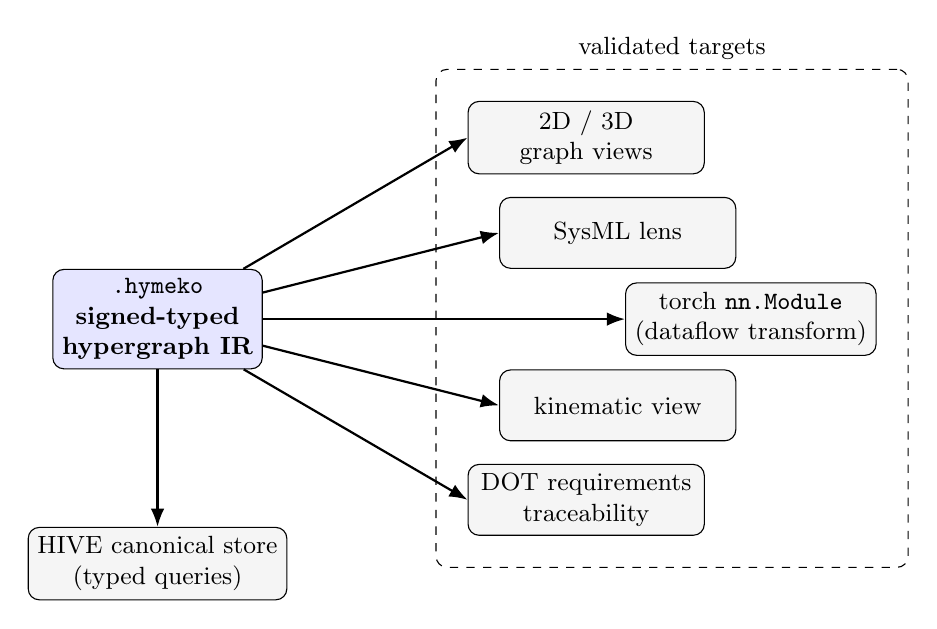
\begin{tikzpicture}[
  >=Latex, node distance=10mm and 20mm,
  src/.style={draw, rounded corners, fill=blue!10, minimum width=26mm,
              minimum height=11mm, align=center, font=\small\bfseries},
  tgt/.style={draw, rounded corners, fill=gray!8, minimum width=30mm,
              minimum height=9mm, align=center, font=\small},
  every edge/.style={draw, ->, thick}
]
  \node[src] (src) {\texttt{.hymeko}\\ signed-typed\\ hypergraph IR};

  \node[tgt, above right=12mm and 26mm of src] (views) {2D / 3D\\ graph views};
  \node[tgt, above right=0mm and 30mm of src]  (sysml) {SysML lens};
  \node[tgt, below right=0mm and 30mm of src]  (kin)   {kinematic view};
  \node[tgt, right=46mm of src]                (nn)    {torch \texttt{nn.Module}\\(dataflow transform)};
  \node[tgt, below right=12mm and 26mm of src] (dot)   {DOT requirements\\ traceability};
  \node[tgt, below=20mm of src]                (hive)  {HIVE canonical store\\ (typed queries)};

  \path (src) edge (views.west);
  \path (src) edge (sysml.west);
  \path (src) edge (kin.west);
  \path (src) edge (nn.west);
  \path (src) edge (dot.west);
  \path (src) edge (hive.north);

  \node[draw, dashed, rounded corners, fit=(views)(sysml)(kin)(nn)(dot),
        inner sep=4mm, label=above:{\small validated targets}] {};
\end{tikzpicture}
\caption{One source, many targets. A single \texttt{.hymeko} IR fans out to
graph views, a SysML lens, a kinematic view, a PyTorch \texttt{nn.Module}, a DOT
requirements-traceability graph, and the HIVE canonical store. Each target is a
deterministic compilation of the same IR, so targets cannot drift independently.}
\label{fig:fanout}
\end{figure}

\begin{description}[leftmargin=1.4em,style=nextline]
  \item[2D / 3D graph views] Layout-oriented renderings of the hypergraph for
    inspection and editing.
  \item[SysML lens] A projection of typed vertices and hyperedges onto SysML
    \cite{omgsysml} constructs, so the same IR can be read by a systems engineer
    in familiar notation.
  \item[Kinematic view] A mechanism/linkage projection for the CPS-physical part
    of the model.
  \item[PyTorch \texttt{nn.Module}] The IR is compiled, as a dataflow transform,
    into a neural module whose computation graph mirrors the hypergraph. This is
    the ``neural target'' exercised empirically in Section~8.
  \item[DOT requirements traceability] A Graphviz DOT graph linking requirements
    to the IR elements that satisfy them.
  \item[HIVE canonical store] A canonical store of the IR answerable by typed
    queries, providing a persistent, queryable source of truth.
\end{description}

Because every target is generated from the IR, ``many lenses, one source''
is not a wish but a structural guarantee: there is exactly one editable artifact.

\section{Structural accountability}
\label{sec:accountability}
``Accountable'' is made testable by two mechanisms.

\paragraph{Validation gate.}
Compilation is gated. An IR that fails validation does not emit any target. This
turns malformed or internally-inconsistent models into a hard failure at compile
time rather than a silent, plausible-looking but wrong artifact downstream.

\paragraph{Structural parity.}
For the neural target, accountability is sharpened into a one-to-one
correspondence: each emitted neural submodule must correspond to exactly one IR
layer, and vice versa. The emitted \texttt{nn.Module} is therefore not an opaque
approximation of the IR --- it is a structural image of it, checkable element by
element.

\paragraph{The broken-twin test.}
To show the gate has teeth, the framework includes a deliberately corrupted
``broken twin'' of a valid IR. The twin fails the validation gate and
\emph{refuses to emit}. This is the positive evidence that the gate rejects what
it should: a model that cannot be made structurally accountable does not produce
a target at all, rather than producing one that quietly disagrees with its source.

\section{Hypergraph generators: a parity contribution}
\label{sec:generators}
Testing structural parity requires a supply of hypergraphs with known,
combinatorially exact structure. The framework provides a typed family of
generators, unified behind a single typed enum
(\texttt{HypergraphGenerator}), so that a caller selects a construction by a
typed variant rather than by a string-typed mode. The family covers:

\begin{itemize}[leftmargin=1.4em]
  \item \textbf{Steiner triple systems} $S(2,3,n)$, a classical design in which
    every pair of points lies in exactly one block (triple). Three constructions
    are provided according to $n$:
    \begin{itemize}[leftmargin=1.4em]
      \item the canonical \textbf{Fano plane} for $n=7$;
      \item the closed-form \textbf{Bose construction} for $n \equiv 3 \pmod 6$;
      \item a \textbf{most-constrained-pair (MRV) backtracking} search for
        $n \equiv 1 \pmod 6$.
    \end{itemize}
  \item \textbf{Sunflowers} ($\Delta$-systems): families of sets sharing a common
    core, used as a controlled-overlap stress structure.
  \item \textbf{Complete $r$-uniform hypergraphs} $K_n^{(r)}$: all $r$-subsets of
    an $n$-set, a dense reference structure.
\end{itemize}

The single enum dispatches to the correct construction, so adding a new
generator means adding a variant, not a new free-function family. \textbf{22
in-crate tests pass} for this generator family.

\section{P-graph methodology}
\label{sec:pgraph}
The framework includes a Process-graph (P-graph) methodology, \emph{available as
infrastructure} (we do not claim it has been applied to the vision study).
Specifically it provides:
\begin{itemize}[leftmargin=1.4em]
  \item the Friedler P-graph axioms \textbf{A1--A5} \cite{friedler1992};
  \item \textbf{Maximal Structure Generation (MSG)} and \textbf{Solution
    Structure Generation (SSG)};
  \item the \textbf{Accelerated Branch-and-Bound (ABB)} algorithm; and
  \item reachability rules over the process structure.
\end{itemize}
This methodology is validated against the worked examples in the Friedler
P-graph textbook. We state it here as a capability of the framework, not as a
component of the empirical study below.

\section{Empirical case study: a hypergraph neural target on vision}
\label{sec:empirical}
\textbf{All results in this section are PRELIMINARY and single-seed where so
noted.} They concern the IR's neural target, not a claim about the vision model
as a whole.

\paragraph{Architecture.}
The backbone is a Bochner-wrapped hypergraph-convolution model with three
branches (\emph{walk}, \emph{polygon}, \emph{triangle}). Prior work
\emph{falsified} the bare-sum aggregator that simply summed the branches. The
present study replaces it with a learned-$\alpha_k$ branch mixer, a highway gate
of the form $T \cdot H(m) + (1-T)\cdot s$, and a top-down cross-scale pyramid.
We compare this \emph{upgraded} model against the \emph{baseline} (bare sum) in
three settings.

\paragraph{MNIST classification (3 paired seeds, 4 epochs, CPU).}
Here three paired seeds are used; we report the mean and a paired standard
deviation (pstd). The upgraded model improves the mean test accuracy by
$+11\%$ relative and reduces variance by roughly $5\times$, at a modest
parameter cost.

\paragraph{Cluttered-MNIST detection.}
Two detection settings are reported, both single-seed: a \emph{toy} run
(400 training images, 8 epochs) and a \emph{scale} run (2000 training images,
20 epochs, GPU). The proxy metric is mAP50\_proxy. In the scale run the upgraded
model is \textbf{still climbing at epoch 20}: its last three epoch values are
$0.117$, $0.126$, $0.135$, so $0.135$ is a not-yet-converged final value, not a
plateau.

\begin{table}[ht]
\centering\footnotesize
\setlength{\tabcolsep}{3.2pt}
\begin{tabular}{@{}llrrr@{}}
\toprule
Setting & Model & Metric & Value & Params \\
\midrule
MNIST cls.\ (3 seeds, 4 ep, CPU)    & baseline (bare sum) & mean test-acc & $0.272$ (pstd $0.032$) & $4736$ \\
MNIST cls.\ (3 seeds, 4 ep, CPU)    & upgraded            & mean test-acc & $0.303$ (pstd $0.006$) & $5811$ \\
\midrule
Clutter-MNIST det.\ toy (400 img, 8 ep)   & baseline & final mAP50\_proxy & $0.022$ & --- \\
Clutter-MNIST det.\ toy (400 img, 8 ep)   & upgraded & final mAP50\_proxy & $0.085$ & --- \\
\midrule
Clutter-MNIST scale (2k img, 20 ep, GPU) & baseline & final mAP50\_proxy & $0.106$ & $4821$ \\
Clutter-MNIST scale (2k img, 20 ep, GPU) & upgraded & final mAP50\_proxy & $0.135$ & $5896$ \\
\bottomrule
\end{tabular}
\caption{Preliminary results. MNIST classification is over 3 paired seeds
(mean, pstd); both detection rows are single-seed. The baseline detection
``scale'' value $0.106$ is saturated by $\sim$epoch~11; the upgraded
``scale'' value $0.135$ is still climbing at epoch~20 (last three epoch
values $0.117, 0.126, 0.135$). Relative improvements: $+11\%$ mean on MNIST
classification; $\sim\!4\times$ on toy detection; $+27\%$ on scale detection.}
\label{tab:results}
\end{table}

\paragraph{Honest conclusions.}
We state the following plainly.
\begin{enumerate}[leftmargin=1.6em]
  \item[(a)] The upgrade \emph{consistently} beats the bare-sum aggregator across
    all three settings (MNIST classification, toy detection, scale detection).
  \item[(b)] It does \textbf{not} overturn the vision falsification. Both
    detection numbers are below the prior config-F headline of $0.174$ (measured
    at $5000$ training images / $20$ epochs); and on MNIST classification a
    trivial $\mathrm{Linear}(784,10)$ reaches $\sim\!0.91$ while these sit at
    $\sim\!0.30$.
  \item[(c)] The per-image hypergraph construction (quadtree $\to$ stimulus graph
    $\to$ Forman--Ricci curvature $\to$ Hodge Laplacian) is CPU-bound, so the GPU
    did not materially speed training. A \emph{topology cache} --- reusing the
    per-image graph across epochs, since it is geometry-determined --- is the
    planned enabler for the full $5000$-image / $40$-epoch run.
  \item[(d)] The untested axis is \emph{brain-predictivity} (Cichy-92 fMRI), not
    classification accuracy.
\end{enumerate}

\section{Related work}
\label{sec:related}
HyMeKo's IR builds on hypergraph theory \cite{berge1973} and on the recent line
of hypergraph neural networks, in particular HGNN \cite{feng2019}. The neural
target draws on Kolmogorov--Arnold networks \cite{liu2024kan}, and on
discrete-geometric notions of curvature and flow: combinatorial / Forman Ricci
curvature \cite{forman2003} and stochastic discrete Ricci flow rewiring (SDRF)
\cite{topping2022}. The P-graph methodology follows the Friedler axioms
\cite{friedler1992}. The SysML lens targets the OMG SysML standard
\cite{omgsysml}.

\section{Conclusion and future work}
\label{sec:conclusion}
The contribution of this work is infrastructure: a single canonical
signed-typed hypergraph IR that compiles, under a validation gate and a
structural-parity check, to many faithful targets, so that a CPS model is one
accountable object rather than $N$ drifting artifacts. The empirical study is
honest about its limits --- the upgraded neural target consistently beats the
falsified bare-sum aggregator, but does not overturn the standing vision
falsification at the scales we can afford.

Future work follows three lines. First, the \emph{topology cache} that turns the
CPU-bound per-image hypergraph construction into a one-time cost, enabling the
full $5000$-image / $40$-epoch tuned run. Second, using the P-graph SSG/ABB
machinery (Section~\ref{sec:pgraph}) as a principled, structure-aware search over
architecture structure rather than ad-hoc tuning. Third, broadening the transform
targets beyond those in Section~\ref{sec:targets} --- candidate targets include
BehaviorTree.CPP, PDDL, and ROS~2 actions --- so that the same accountable IR can
drive execution as well as analysis.

\begin{thebibliography}{9}
\bibitem{berge1973} C.~Berge. \emph{Graphs and Hypergraphs.} North-Holland, 1973.
\bibitem{feng2019} Y.~Feng, H.~You, Z.~Zhang, R.~Ji, Y.~Gao.
  \emph{Hypergraph Neural Networks.} AAAI, 2019.
\bibitem{liu2024kan} Z.~Liu et al.
  \emph{KAN: Kolmogorov--Arnold Networks.} arXiv preprint, 2024.
\bibitem{forman2003} R.~Forman.
  \emph{Bochner's method for cell complexes and combinatorial Ricci curvature.}
  Discrete \& Computational Geometry, 29(3):323--374, 2003.
\bibitem{topping2022} J.~Topping, F.~Di~Giovanni, B.~P.~Chamberlain, X.~Dong,
  M.~M.~Bronstein. \emph{Understanding over-squashing and bottlenecks on graphs
  via curvature.} ICLR, 2022.
\bibitem{friedler1992} F.~Friedler, K.~Tarj\'an, Y.~W.~Huang, L.~T.~Fan.
  \emph{Graph-theoretic approach to process synthesis: axioms and theorems.}
  Chemical Engineering Science, 1992.
\bibitem{omgsysml} Object Management Group.
  \emph{OMG Systems Modeling Language (SysML).} OMG specification.
\end{thebibliography}

\vspace{0.6em}
\noindent\footnotesize\emph{Note on citations:} bibliographic details follow the
standard references for each method; exact pages, venues and identifiers should
be verified against the project bib files before external use. No DOIs are
asserted here.
\end{document}
